\chapter{Implementácia programu}
V tejto kapitole sa budeme venovať niektorým významnejším črtám implementácie nášho programu, ktorý na vstupe dostane súbor popisujúci evolučnú históriu,
umožní uživateľovi zmeniť niektoré nastavenia a prípadne spustiť optimalizáciu a nakoniec zobrazí grafickú reprezentáciu vstupnej evolučnej histórie podľa
podľa toho aké zmeny vykonal uživateľ. Bližšie sa pozrieme na to v akom formáte má byť zapísaný vstup, ako bude vyzerať výstup, aké kroky vykonájú triedy nášho programu,
akým spôsobom dokáže uživateľ interagovať s programom,
ako aj to ktoré nastavenia vieme meniť a čo reprezentujú.
\section{Vstup}
\label{sec:vstup}
Vstup musí obsahovať dáta, ktoré nám umožnia vykresliť fylogenetický strom, a zobraziť v ňom k akým zmenám v genóme došlo, a ktoré udalosti sú za to zodpovedné.
To znamená že v infromáciách o jednotlivých vrcholov sa budú nachádzať aj poznatky o tom, ako vyzerá genóm daného vrcholu, a aké sú vzťahy medzi týmto a genómom jeho predchodcu.
\subsection{Formát}


\begin{table}[!htb]
\label{tab:vstup}
\begin{center}
\begin{tabular}{llllllll}
predok & e1 & root & 0 & root & 1 2 1 5 4 3 2 & \#  & -1 -1 -1 -1 -1 -1 -1 \\
predok & e2 & e1 &  0.05 & dup &  1 2 1 2 5 4 3 2 & \# & 0 1 2 1 3 4 5 6 \\
clovek & e3 & e2 &  0.12 & sp &   1 2 1 2 5 4 3 2 & \# & 0 1 2 3 4 5 6 7 \\
clovek & e4 & e3 &  0.13 & del & 1 2 1 2 4 3 2 & \# & 0 1 2 3 5 6 7 \\
clovek & e5 & e4 &  0.14 & ins & 1 2 1 6 7 2 4 3 2 & \# & 0 1 2 -1 -1 3 4 5 6 \\
clovek &  e6 & e5 &  0.2 & inv &  1 -1 -2 6 7 2 4 3 2 & \# & 0 2 1 3 4 5 6 7 8 \\
clovek & e7 & e6 &  0.25 & leaf & 1 -1 -2 6 7 2 4 3 2 & \# & 0 1 2 3 4 5 6 7 8 \\
simpanz & e8 & e2  & 0.12 & sp &  1 2 1 2 5 4 3 2 & \# & 0 1 2 3 4 5 6 7 \\
simpanz & e9 & e8 &  0.2 & leaf & 1 2 1 2 5 4 3 2 & \# & 0 1 2 3 4 5 6 7 \\
 \end{tabular}

\end{center}
\caption{Ukážka vymysleného vstupu v súčasnom formáte \cite{biowiki}}
\end{table}

Vstupný súbor nášho programu bude tvoriť postupnosťou riadkov, podobná tej akú vidíme v tabulke  \ref{tab:vstup}.
Každý riadok predstavuje jeden \emph{krok e.h.}.
Prvý riadok je koreňom danej histórie, opisuje prvotný stav sekvencie a má priradenú špeciálnu udalosť "root".
Každý ďalší riadok, opisuje niektorý z nasledujúcich krokov e.h. obsahuje zoznam génov nachádzajúcich sa v tomto kroku
a spolu so svojím predchodcom nám umožnuje určiť aké udalosti z \ref{evhist} viedli k súčasnému stavu.
Predchodca sa v súbore musí nachádzať vždy skôr než nasledovník, aj preto je prvým riadkom koreň.
\newline
Riadok obsahuje niekoľko reťazcov a čísel, oddelených medzerou alebo viacerými medzerami, ak je to potrebné pre lepšiu prehľadnosť.
\paragraph{Význam stĺpcov:}

\begin{description}

\item[Prvý stĺpec] je názov objektu, ktorého sa týka daný riadok.

\item[Druhý stĺpec] je id riadku.

\item[Tretí stĺpec] je id predchodcu, prvý riadok má špeciálne id predchodcu s hodnotou root.

\item[Štvrtý stĺpec] je čas, v ktorom sa daná udalosť odohrala. Koreň sa nachádza v čase 0, a čas je rastúci.

\item[Piaty stĺpec] je skratka niektorej z udalostí, popísaných v sekcii \ref{evhist} pokiaľ sa v danom \emph{kroku e.h.} odohrala iba jedna z týchto udalostí, alebo jedna zo trojice udalostí root/leaf/other.
Root je udalosť slúžiaca na identifikáciu koreňa.
Leaf slúži na určenie času v ktorom sa daná vetva končí, medzi udalosťou označenou ako leaf a jej predchodcom nemuselo prísť k žiadnym zmenám.
Other použijeme ak tento rozdiely medzi týmto a predchádzajúcim krokom niesme schopný popísať pomocou jednej udalosti,
znamená to že takýto krok vznikol kombináciou viacerých udalostí ako napríklad dve duplikácie nasledujúce po sebe alebo translokácia s následnou deléciou.

\item [Nasledujúce stĺpce] obsahujú postupnosť génov. Každý gén je celé číslo, pričom znamienko určuje jeho orientáciu. To znamená že gén 2 je rovnaký ako gén -2, iba opačne orientovaný v rámci dna.

\item [Znak \#] slúži ako ukončenie zoznamu génov.

\item[Zvyšné stĺpce] pre každý gén určujú poradie predka génu v predchodcovi jeho riadku. Ak tento gén nemá predchodcu, obsahuje riadok hodnotu -1.
Napríklad pre gén 2 z riadku e4 vieme, že poradie jeho predchodcu má index 3. Keďže predchodcom e4 je e3 vieme spojiť štvrtý (indexujeme od nuly) gén z riadku e3 s štvrtým génom (gén 2) riadku e4.

\end{description}

\begin{table}[!htb]
\label{tab:vstup}
\begin{center}
\begin{tabular}{llllllll}
predok & e1 & root & 0 & root & 1 2 1 5 4 3 2 & \#  & -1 -1 -1 -1 -1 -1 -1 \\
predok & e2 & e1 &  0.05 & dup &  1 2 1 2 5 4 3 2 & \# & 0 1 2 1 3 4 5 6 \\
clovek & e3 & e2 &  0.12 & sp &   1 2 1 2 5 4 3 2 & \# & 0 1 2 3 4 5 6 7 \\
clovek & e4 & e3 &  0.13 & del & 1 2 1 2 4 3 2 & \# & 0 1 2 3 5 6 7 \\
clovek & e5 & e4 &  0.14 & ins & 1 2 1 6 7 2 4 3 2 & \# & 0 1 2 -1 -1 3 4 5 6 \\
clovek &  e6 & e5 &  0.2 & inv &  1 -1 -2 6 7 2 4 3 2 & \# & 0 2 1 3 4 5 6 7 8 \\
clovek & e7 & e6 &  0.25 & leaf & 1 -1 -2 6 7 2 4 3 2 & \# & 0 1 2 3 4 5 6 7 8 \\
simpanz & e8 & e2  & 0.12 & sp &  1 2 1 2 5 4 3 2 & \# & 0 1 2 3 4 5 6 7 \\
simpanz & e9 & e8 &  0.2 & leaf & 1 2 1 2 5 4 3 2 & \# & 0 1 2 3 4 5 6 7 \\
 \end{tabular}

\end{center}
\caption{Ukážka vymysleného vstupu v súčasnom formáte \cite{biowiki}}
\end{table}

\section{Návrh výstupu}
\label{sec:vykreslene}
\begin{figure}
\centerline{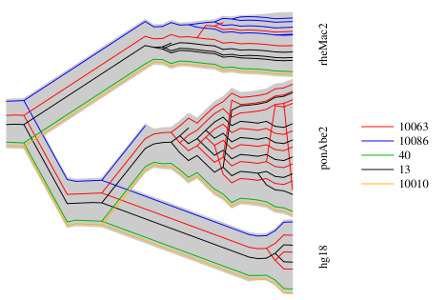
\includegraphics[width=1\textwidth]{images/DUP-tube-tree}}
\caption{Možné zobrazenie histórie, Zdroj:\cite{Vinar2010}}\label{obr:tree}
\end{figure}
Výstupom nášho programu by nemal byť iba jednoduchý fylogenetický strom, keďže naším cielom je zobraziť 
kompletnú informáciu o génoch ktoré sa nachádzajú v evolučnej histórii.
Potrebujeme preto nájsť spôsob akým túto informáciu pridať do fylogenetického stormu.
Rozhodli sme sa teda, že každý gén bude zobrazený počas celej jeho existencie v evolučnej histórii. Naše zobrazenie evolučnej histórie bude perdstavovať
les stromov, v ktorom jednotlivé stromy reprezentujú gény nachádzajúce sa v týchto druhoch. 

\emph{X-ová} os slúži ako os času, naľavo sa nachádza čas 0, ktorý postupne rastie tak, aby sa do obrázku zmestil aj najneskorší krok evolučnej histórie.

\emph{Gény} sú znázornené farebnými čiarami, ktoré idú vodorovne až kým sa nedostanú do bodu v ktorom má nastať udalosť.
Ak vieme že nasledujúci krok $k$ evolučnej histórie sa nachádza v čase $t_k$, tak gény dojdú bez zmeny do bodu $t_k - d$,
kde $d$ reprezentuje čas potrebný pre odohratie zmien. Zmeny vedúce ku kroku $k$ sa teda udejú počas časového rozmedzia $t_k - d$ až $t_k$.
Pozícia génov v rámci Ypsilonovej osi je v udalosti root daná ich reálnym poradím, prvý gén udalosti root sa nachádza najvyššie na Y osi.
Pre každý ďalší krok platí, že gény daného kroku sú na Y osi zoradené podľa poradia v akom sa nachádzajú v tomto kroku evolučnej histórie.

\emph{Duplikáciu}, teda skopírovanie jedného alebo viacerých génov zobrazíme tak, že každý zo stromov reprezentujúci zduplikované gény rozvetvíme. 
Vetvenie začne v čase $t_k - d$.

Speciáciu by sme v klasickom druhovom strome zobrazili ako rozvetvenie druhového stromu, počas speciácie teda rozvetvíme všetky gény tak ako by sa nachádzli v rozvetvení druhového stromu 
- získame dve sady vetiev reprezentujúce naše gény.
Rozdiel medzi speciáciou a duplikáciou ktorá prebehla na celom genóme je zreteľný vo vzdialenosťi na Y osi, kedy pri speciácii rozoznávame dve oddelené sady vetiev, ktoré sú od seba dostatočne vzdialené,
zatiaľ čo duplikácia by vytvorila iba jednu sadu vetiev. Ak sa jedna vetva speciácie nachádza v čase $t_a$ a druhá v čase $t_b$ zobrazíme 
začiatok speciácie do času $t_x - d$ kde $t_x$ je skorší z časov $t_a,t_a$.

Inzerciu génov znázorneníme pridaním nového stromu pre každý vložený gén, začiatok pridaních stromov sa nachádza v čase $t_k$.

Deléciu génu zobrazíme ako ukončenie vetvy stromu, ktorá reprezentovala inštanciu tohto génu, takúto vetvu ukočíme v čase $t_k - d$.

Translokáciu zobrazíme ako kríženie vetiev translokovaných génov tak, aby sa po tomto krížení nachádzali vetvy v správnom poradí,
kríženie sa začne v čase $t_k - d$ a skončí v čase $t_k$.

Inverziu znázorníme podobne ako translokáciu, avšak keďže pri inverzii okrem zmeny poradia génov dochádza aj k zmene ich orientácie, pridáme do zobrazenia údaj o orientácii génu.
Gén so zmenenou orientáciou nebudeme zobrazovať plnou čiarou, na miesto nej využijeme prerušovanú čiaru. To nám umožní zobraziť inverziu jedného génu,
ktorá by inak nemusela byť viditeľná a inverziu dvoch génov ktorú by sme si mohli v niektrých prípadoch pomýliť s translokáciou. Zmena štýlu čiari nastáva už v čase  $t_k - d$.

Root je začiatok pre všetky stromy génov, ktoré sa nachádzajú v počiatočnom predkovi.

Leaf ukončí vetvi génov v čase $t_k$.\newline
Obrázok \ref{obr:events} ilustruje všetky udalosti ktoré sme si práve opísali, naľavo sa nachádza krok evolučnej histórie "root" obsahujúci štyri gény,
nasleduje inzercia dvoch ďalších génov a po nej speciácia. Pri speciácii vzniknú dve vetvy génov ktoré sú od seba dostatočne vzdialené na to aby sme ich rozoznali.
Navyše vrchná vetva speciácie sa začína v neskoršom čase, potom už neobsahuje žiadne udalosti iba končím v liste.
V spodnej vetve sa odohráva inverzia, po nej translokácia, nakoniec delécia dvoch génov a ukončenie zvyšných v liste.
\begin{figure}
\centerline{\includegraphics[width=1\textwidth]{images/udalosti}}
\caption{Príklad zobrazenia histórie naším programom}\label{obr:events}
\end{figure}
\section{Triedy programu}
V stručnosti si predstavíme základne funkcie ktoré plnia triedy v našom programe bez toho, aby sme zachádzali príliš hlboko do implementačných detailov.
\paragraph{Bak} je hlavnou triedou ktorá sa nachádza v našom programe.
Načíta vstupné parametre, a na ich záklda sa rozhodne či program prebehne neinteraktívne, iba na základe prvotného vstupu, 
alebo sa spustí interaktívna grafická aplikáciá využívajúcá JavaFX, ktorá je zapísaná v tejto triede.
\paragraph{EvolutionTree} je kľúčovou triedou celého projektu, reprezentuje evolučnú históriu, obsahuje výpočty potrebné pre jej vykreslenie ako aj optimalizáciu. Obsahuje podtriedu \emph{EvolutionNode} 
ktorá popisuje jeden krok evolučnej histórie. Táto trieda dostane vstupnú históriu a tú si uloží v potrebnom formáte.
Pre každý krok evolučnej histórie si vytvorí jeden \emph{EvolutionNode}, krok typu \emph{root} si priamo uloží a zvyšné kroky si namapuje podľa ich $id$.

Pri vykreslovaní zisťuje, akú šírku bude krok zaberať na obrázku. Pre list je táto šírka daná súčtom šírok jeho génov a medzier medzi nimi. 
Pre zvyšné kroky je daná buď ako ich vlastná šírka, to znamená výpočet rovnaký ako pri liste, alebo ako šírka kroku ktorý po ňom nasleduje, vyberáme väčšiu z hodnôt.
Pokiaľ v kroku nastáva vetvenie druhového stromu, vyberieme ako jeho šírku väčšiu z hodnôt jeho vlastnej šírky, alebo súčtu šírok krokov ktoré z neho vychádzajú, a medzery, ktorú medzi nimi musíme nechať.
Keď pozná šírky ktoré potrebujú jednotlivé kroky môže vykresliť našu evolučnú históriu.

V tejto triede taktiež prebieha aj hľadanie blokov \ref{blok} a následné riešenie problému množinového pokrytia greedy algoritmom alebo jeho export vo forme celočíselného lineárneho programu.
Bloky hľadáme pre každú dvojicu predchodca kroku,krok zvlášť. Pokiaľ je nejaký krok predchodcom pre dva kroky, to znamená že z neho vychádzajú dve speciácie, hľadáme bloky nezávisle pre oboch jeho nasledovníkov.
\paragraph{DrawFactory} je abstraktná trieda slúžiaca pre vykreslovanie evolučnej histórie. V našom programe sa nachádza dve triedy ktoré ju rozširujú.
\emph{FXDrawFactory} slúži na vykreslenie evolučnej histórie v našej JavaFX aplikácii. \emph{SVGDrawFactory} slúži na vykreslenie evolučnej histórie vo formáte \emph{svg} - škálovateľná vektorová grafika, históriu v tomto formáte vieme následne vyexportovať.
\emph{EvolutionTree} dostane inštanciu jednej z týchto dvoch tried a pomocou nej vykreslí evolučnú históriu.
\paragraph{Gene Meta} reprezentuje nastavenia jedného génu, spôsob ako ich exportovať do XML a tiež možnosť načítať takéto nastavenia z XML súboru.
\paragraph{Settings} V tejto triede sa nachádzajú globálne nastavenia ktoré využívame pre vykreslovanie, sú tu uložené aj \emph{GeneMeta} pre niektoré gény,
pokiaľ pre gén neexistujú \emph{GeneMeta}, alebo neobsahujú hodnotu pre požadované nastavenie, využije sa všeobecná hodnota tohto nastavenia ktorá sa nachádza v triede \emph{Settings}.
Trieda \emph{Settings} taktiež obsahuje omožnosť vyexportovať nastavenia, vrátane vrátane všetkých \emph{GeneMeta}, do XML, ako aj možnosť nastavenia z XML súboru načítať.

\section{Ovládanie programu}
Náš program ponúka dve možnosti ako ho ovládať. Prvou z nich je grafická aplikácia ktorá uživateľovi umožnuje interagovať s nastaveniami a spúštať funkcie ktoré náš program obsahuje.
Druhou možnosťou je vložiť nášmu programu všetky požiadavky, ktoré má splniť v príkazovom riadku už pri jeho spustení, tento spôsob nevyžaduje žiadnu ďalšiu interakciu a je ideálny pri potrebe spracovať väčšie množstvo vstupov.
Teraz sa pozrieme na to aké možsnosti ovládania tieto dve alternatívy ponúnkajú.
\subsection{Grafická aplikácia}
\begin{figure}[t]
 \centering
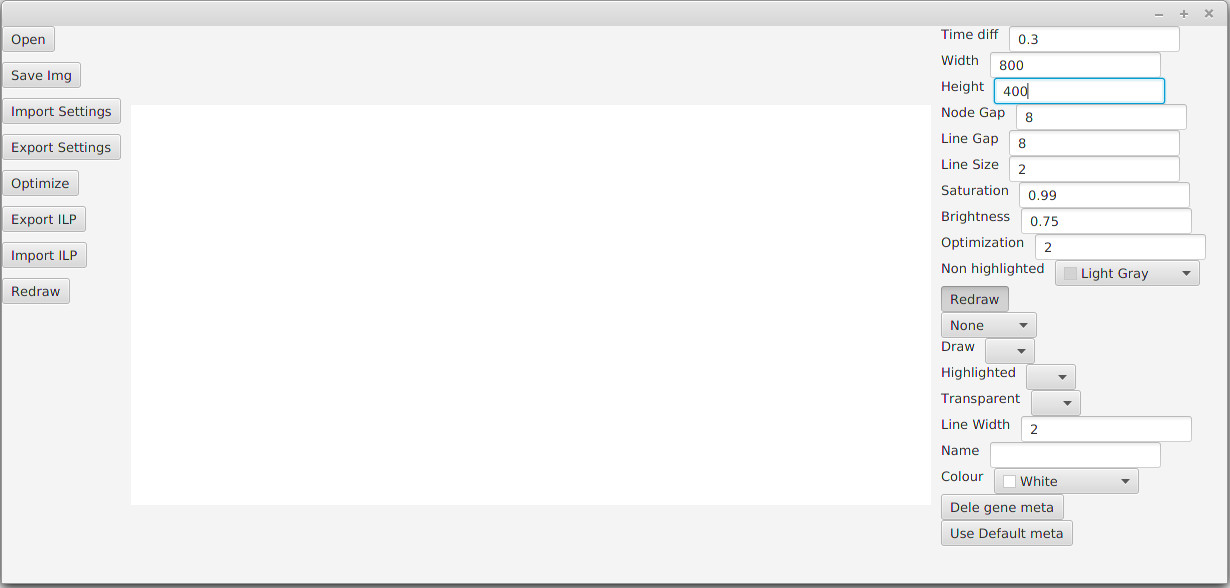
\includegraphics[width=1\textwidth]{images/gui}
\caption{Vzhľad grafickej aplikácie}\label{obr:gui}
\end{figure}

Na obrázku \ref{obr:gui} vidíme základné okno našej aplikácie. V strede sa nachádza plocha na ktorú sa vykresľuje evolučná história. Na ľavo sa nachádza základná sada tlačidiel a na pravo ovládacie prvky pre zmenu nastavení.
Štandardne má aplikácia pri spustení rozmery 1200x800 a plocha, na ktorú sa vykresluje rozmery 800x800.
\paragraph{Tlačidlá na ľavej strane} slúžia k základnému ovládaniu nášho programu, predstavíme si čo ktoré tlačidlo po stlačení vykoná, a aké to má využitie.

\emph{Open} otvorí nové okno ktoré nám umožní zvoliť súbor ktorý cheme otvoriť, tento súbor by mal byť vo formáte popísanom v sekcii \ref{sec:vstup}. 
 Zvolená evolučná história sa načíta a vykreslí.
 
\emph{Save img} otvorí nové okno ktoré nám umožní zvoliť si do akého súboru sa uloží náš súčasný obrázok, ten sa ukladá vo formáte SVG.

\emph{Import Settings} v novom oknem nám umožní vybrať si súbor vo formáte XML obsahujúci nastavenia ktoré má načítať.

\emph{Export Setting} umožnuje vybrať súbor do ktorého sa uložia naše nastavenia. Nastavenia sa ukladajú vo formáte XML.

\emph{Optimize} zostrojí problém množinového pokrytia tak ako je to popísané v kapitole \ref{chap:setcover} a následne ho približne vyrieši pomocou greedy algoritmu.
poďla toho akú hodnotu má pole \emph{optimization} sa toto riešenie prenesie do zobrazenia.

\emph{Export ILP} podobne ako tlačidlo \emph{Optimize} zostrojí problém množinového pokrytia, ale miesto toho aby našiel jeho približné riešenie,
uloží ho zapísaný ako celočíselný lineárny program, do nami zvoleného súboru. Súbor do ktorého sa uloží vyberáme už klasicky v novom okne ktoré nám otvorí.

\emph{Import ILP} v novom oknem nám opäť umožní zvoliť súbor ktorý sa otvorí, tento krát má však daný súbor obsahovať riešenia celočíselného lineárneho programu.
 Náš program je nastavený tak aby vedel spracovať riešenia ktoré produkuje \emph{CPLEX}, to akým spôsobom sa načítané riešenie prenesie do zobrazenia evolučnej histórie, opäť záleží na tom,
 aká hodnota sa nachádza v poli \emph{optimization}.
 
\emph{Redraw} po stlačení tohto tlačidla dojde k prekresleniu obrázku.
\paragraph{Ovládacie prvky na pravej strane}
Na ľavej strane sa nachádzajú dve sady ovládacích prvkov. Prvá sada mení nastavenia ktoré sa nachádzajú priamo v triede \emph{Settings} a sú zdielané všetkými génmi a celým prostredím.
Druhá sada mení nastavenia špecificky pre zvolený gén, je to teda spôsob akým meníme nastavenia triedy \emph{GeneMeta} pre konkrétny gén.
\paragraph{Globálne}\mbox{}\linebreak
\emph{Time diff}je číslo vyjadrujúce koľko času má zabrať odohranie udalosti na X-ovej osi, ak má krok evolučnej histórie $k$ známy čas $t_k$ tak 
jeho udalosť sa začne odohrávať už v čase $t_k - \emph{Time diff}$, tento čas však nesmie byť menší ako čas v ktorom sa odohral predchodca kroku $k$. Time diff reprezentuje rovnakú premenn=u ako znak $d$ v sekcii \ref{sec:vykreslene}. 

\emph{Width} určuje dĺžku X-ovej osi, teda šírku nášho obrázku, náš program každú evolučnú históriu naškáluje tak, aby ležala na celej tejto osi.

\emph{Height} určuje dĺžku Y osi, teda výšku nášho obrázku, náš program na šírku neškáluje, to aká časť šírky je pokrytá závisí od šírok génov a ich medzier.

\emph{Node Gap} určuje vzdialenosť medzi dvoma sadami vetiev ktoré vznikli počas speciáce. zadáva sa celé číslo.

\emph{Line Gap} určuje medzeru medzi dvoma susednými génmi ktoré sa nachádzajú v jednom kroku evolučnej histórie.

\emph{Line Size} šírka čiary znázornujúcej jeden gén, platí pre všetky gény pokiaľ nemajú svoje vlastné špecifické nastavenie.

\emph{Saturation} a \emph{Brightness} . Štandardne získavame farby ktoré priradíme génom z modelu HSB - hue,saturation,brightness - slovensky odtieň,sýtosť,jas.
Odtieň v tomto modeli je daný v stupňoch hodnotou $0^\circ-360^\circ$. Rovnomerne rozdeliť odtiene medzi našich $n$ génov,
 je teda rovnaký problém ako rozdeliť kružnicu na $n$ rovnakých častí. Sýtosť a jas sú potom pre všetky gény rovnaké, určujeme ich reálnym číslo z rozmedzia $<0,1>$ .

\emph{Optimization} určuje akým spôsob sa prejaví optimalizácia na výslednom zobrazení evolučnej histórie.Pri hodnote 2 sa génom, ktoré sa nenachádzajú v riešení nastaví atribút $higlighted=false$, vykreslia sa farbou ktorá je daná ako \emph{Non highlighted},
takéto nastavenie vidíme na obrázku \cite{obr:opt} v okinenku číslo 2. Pri hodnote 1 sa nezvolením génom nastaví atribút $trasnparent=true$, zobrazia sa priesvitne, rovnako ako v okienku číslo 3.
Pri hodnote 0 sa nezvolením génom nastaví atribút $draw=false$, a teda sa nezobrazia vôbec, rovnako ako štvrtom okienku. Génom ktoré sa nachádzajú v riešení sa atribúty nemenia ani v jednom z týchto nastavení.

\emph{Non highlighted} umožnuje výber farby pre gény, ktoré nie sú zvýraznené. To sú tie pre ktoré $highlighted=false$ a zároveň $draw=true$ a $transparent=false$. Tieto hodnoty génom manuálne nastavíme alebo ich získajú pokiaľ sa nenachádzajú v riešení optimalizácie a $optimize=2$.

\emph{Redraw} je preínač, pokiaľ je zapnutý obrázok sa automaticky prekreslí po tom, čo zmeníme niektoré z jeho nastavení. 
V opačnom prípade obrázok prekreslíme stlačením ľavého tlačidla \emph{redraw}
\paragraph{Špecifické pre gén} sa aplikujú na vybraný gén ktorý zvolíme z rozklikávacieho listu.
V tomto liste sa nachádzajú vśetky gény z histórie, bez ohľadu na to, či pre ne existuje záznam \emph{GeneMeta} uložení v nastaveniach \emph{Settings}.
Okrem toho sa v liste nachádzajú dve špecíalne hodnoty. \emph{None} vyjadruje že nemáme zvolený žiaden gén a nebudeme vedieť meniť žiadne nastavenia špecifické pre gén.
\emph{Default} slúži k nastaveniu hodnôt, ktoré využívajú všetky gény bez vlastných \emph{GeneMeta}. Pre \emph{Default} nevieme nastavovať \emph{Name} ani \emph{Colour}.
Pokiaľ si z listu zvolíme gén ktorý nemá vlastný záznam \emph{GeneMeta}, tento záznam sa vytvorí až keď tomuto génu nastavíme niektorú z hodnôt.
Do polí \emph{Draw,Transparent a Highlighted} sa prekopíruje hodnota nastavená v \emph{Default}, zvyšné polia môžu zostať prázdne. Pre prázdne polia sa aj naďalej využívajú hodnoty z \emph{Default}.

\emph{Draw} boolean prepínač, hodnota určuje či sa gén vykreslí.

\emph{Transparent} boolean prepínač, pokiaľ sa má gén vykresliť $(draw=true)$, tak hodnota \emph{Transparent} určí, či bude priesvitný $transparent=true$, kedy gén nevidíme, ale zaberá miesto.
Alebo bude nepriesvitný, kedy farbu získa v závislosti od hodnoty \emph{Highlighted}.

\emph{Highlighted} pokiaľ sa má gén nepriesvitne vykresliť $draw=true,transparent=false$ highlighted rozhodujem o tom či bude zvýraznený.
Ak je zvýraznený zobrazí sa s farbou ktorú má nastavenú v \emph{Colour}, v prípade že nemá nastavenú vlastnú farbou použije predpočítanú farbu. Ak nieje zvýraznený použije farbu nastavenú v \emph{Non Highlighted}. 

\emph{Line Width} umožnuje individuálne nastavenie šírky génu. Vkladáme celé číslo.

\emph{Name} je textové pole v ktorom môžme génu nastaviť jeho meno.

\emph{Colour} ponúka výber farby špeciálne pre daný gén.

\emph{Delete gene meta} odstráni záznam \emph{GeneMeta} pre práve zvolený gén.Nefunguje pre \emph{Default}.

\emph{Delete all meta} odstráni všetky existujúce záznamy \emph{GeneMeta} okrem záznamu \emph{Default}.